\documentclass[12pt]{article}

\usepackage[a4paper,margin=1in]{geometry}
\usepackage{amsmath,amssymb}
\usepackage{graphicx}
\usepackage{booktabs}
\usepackage{array}
\usepackage{tcolorbox}
\usepackage{hyperref}
\usepackage{siunitx}
\usepackage{enumitem}
\usepackage{titlesec}
\usepackage{xcolor}
\usepackage{float}
\usepackage{microtype}
\usepackage{tabularx}
\usepackage{colortbl}
\usepackage{xcolor}
\usepackage{pifont} % for \ding symbols
\usepackage{enumitem}

\usepackage[T1]{fontenc}
\usepackage{mathpazo}
\linespread{1.05}
% Colors
\definecolor{secblue}{HTML}{2B4A6F}
\definecolor{lightgray}{HTML}{F2F2F2}
\definecolor{rulecolor}{HTML}{CCCCCC}
\definecolor{warnred}{HTML}{8B2500}

\hypersetup{
    colorlinks=true,
    linkcolor=secblue,
    urlcolor=secblue
}

\titleformat{\section}
  {\Large\bfseries\color{secblue}}
  {\thesection}{0.6em}{}[\vspace{2pt}\color{rulecolor}\hrule\vspace{4pt}]

\titleformat{\subsection}
  {\large\bfseries\color{secblue!80}}
  {\thesubsection}{0.5em}{}

\setlist{itemsep=2pt, topsep=4pt}

\title{\vspace{-1cm}\textbf{\LARGE Zac's Climbing Wall}\\[6pt]
\large Is the Support System Safe?\\[8pt]}
\date{\vspace{-1.6cm}March 2026}

\begin{document}
\maketitle
\vspace{-0.5em}
\textbf{Engineering estimate only. Not a substitute for professional inspection.}

\vspace{1em}

Zac built an inclined climbing wall for bouldering in his backyard. Using a crank mechanism, he rotated it 40 degrees away from the vertical axis. Three ratchet straps secure the top of the board to anchors in a boundary wall.

Only one climber uses the wall at a time. The climber boulders up and down the board. If they fall, they drop onto a mat below.

\textit{What forces do the three straps experience, and how safe is the system?}

\begin{figure}[H]
    \centering
    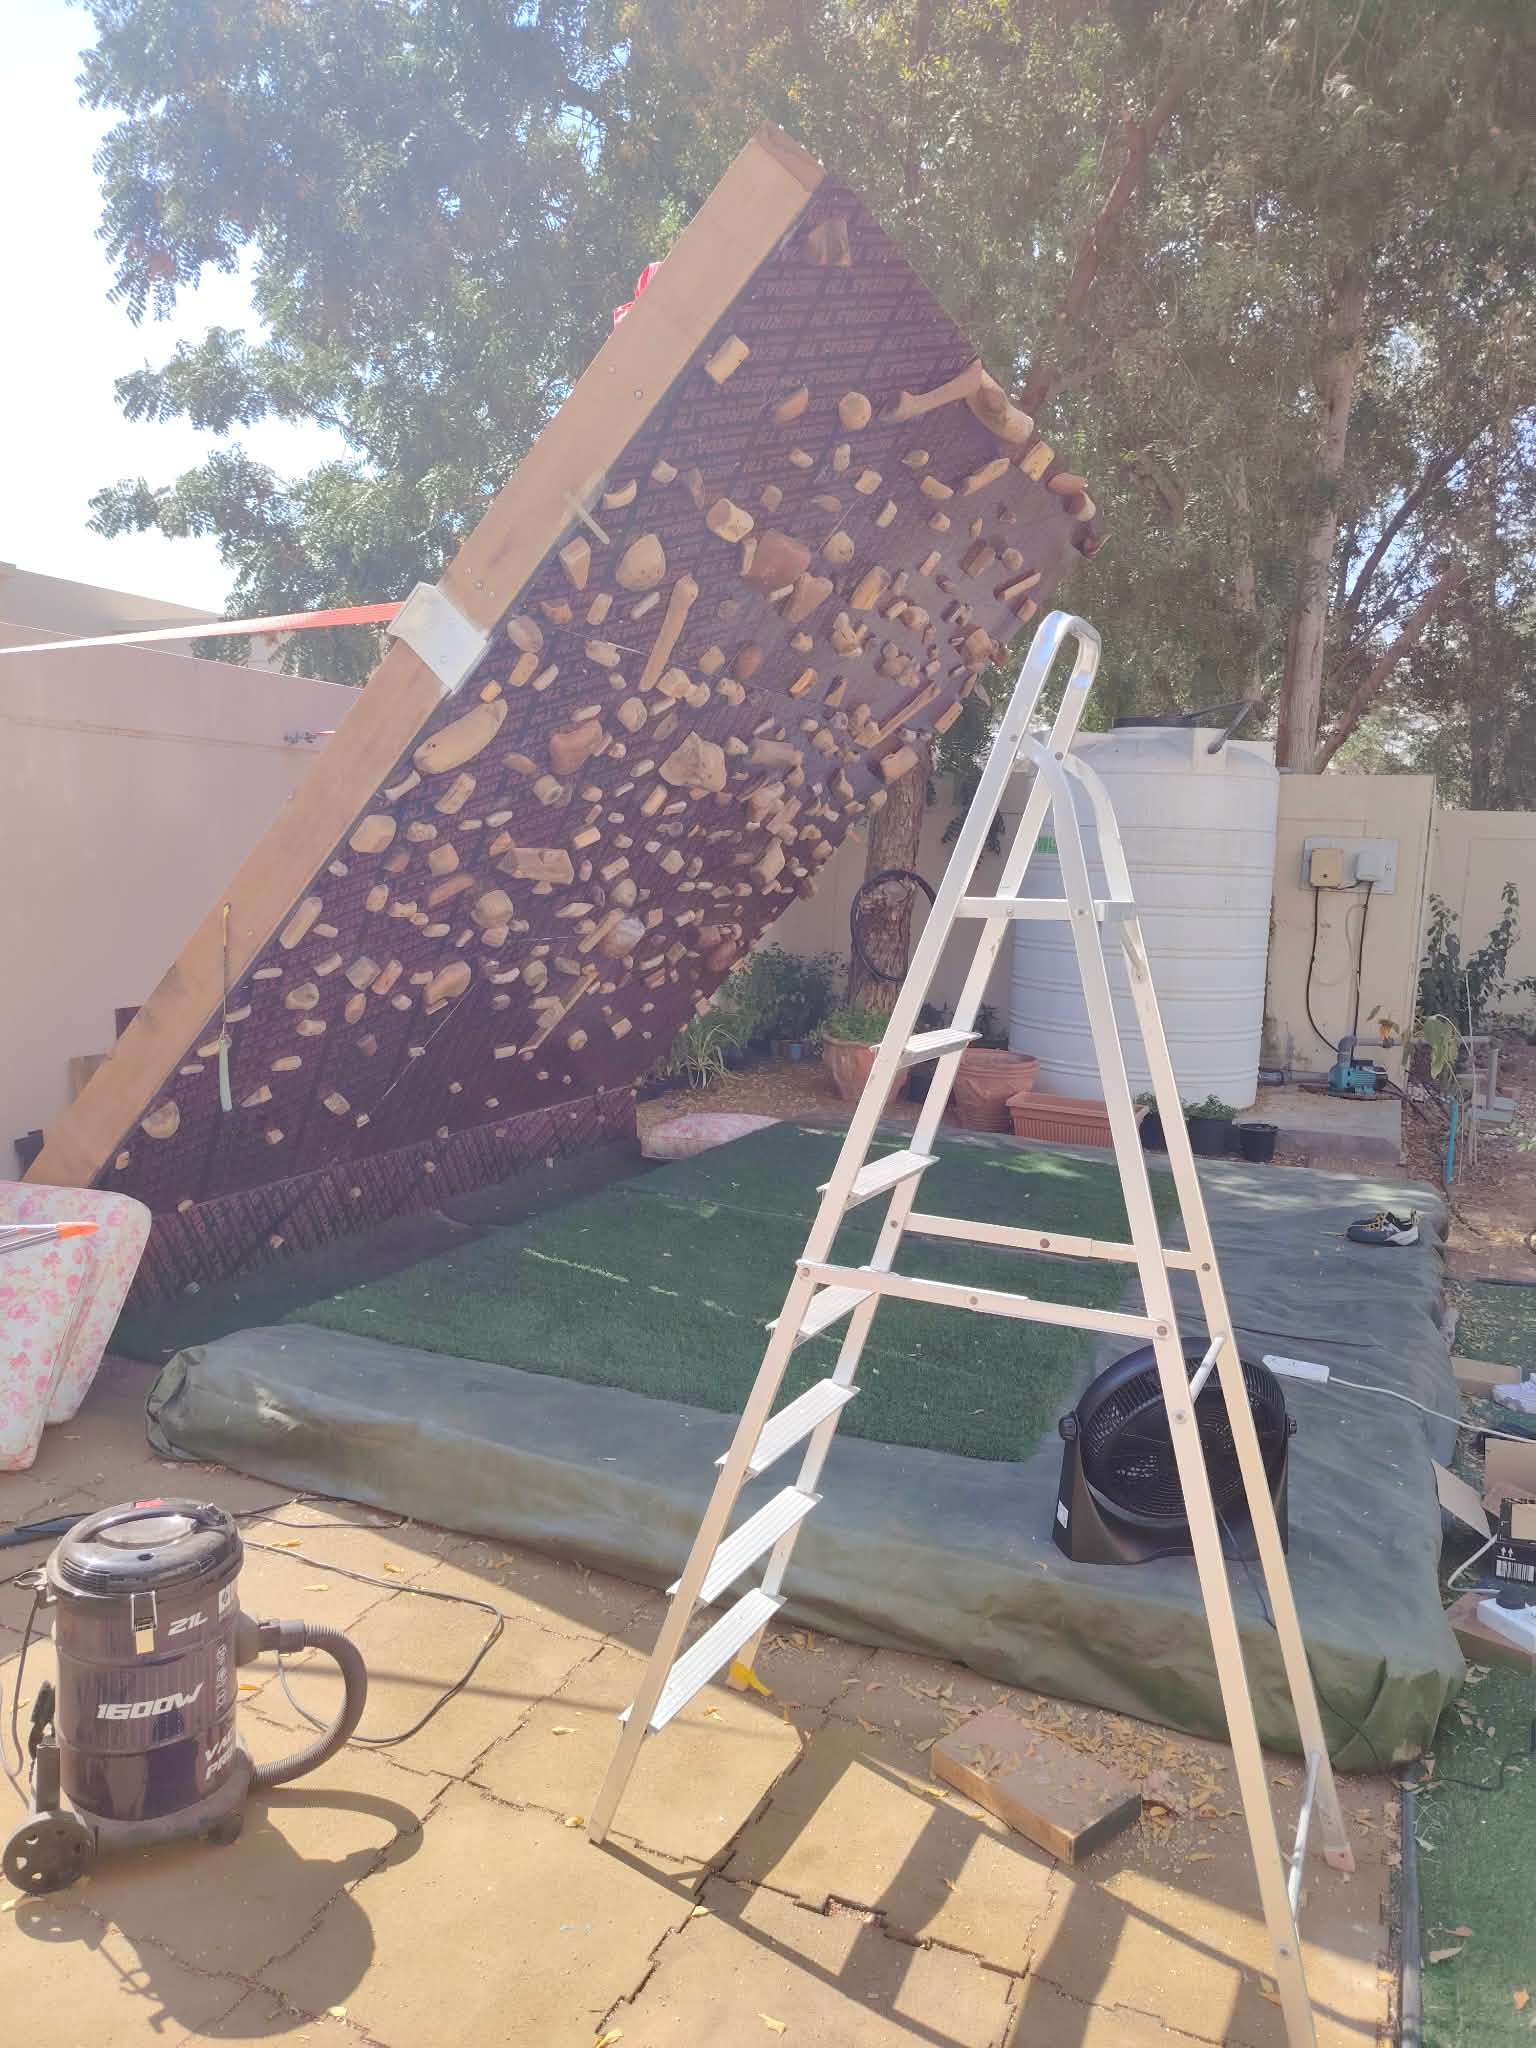
\includegraphics[width=0.5\linewidth]{99a25b7e-b9b8-469f-a854-f97e717b49d8.jpeg}
    \caption{the wall :)}
    \label{fig:wall}
\end{figure}

% =====================================================
\newpage
\section*{Disclaimer}
\addcontentsline{toc}{section}{Disclaimer}

This is an engineering estimate, not a formal structural certification. Full list of limitations in Section~\ref{sec:limitations}.

\newpage
\tableofcontents
% =====================================================
\newpage\section{The Setup}
\label{sec:setup}

A wooden board (366 cm long, 20 cm deep) leans away from a boundary wall. The base rests on a 20~cm $\times$ 32~cm block on the ground (pivot), 54~cm from the wall face. Three ratchet straps near the top of the board connect to eye bolts embedded in the wall at 200~cm above ground.

The boundary wall is 226~cm tall, solid concrete block with rebar tying it into a concrete base, extending at least 60~cm below grade. The nearest corner or gate post is 494~cm to the left and 380~cm to the right of the anchors.
\vspace{0.5em}
\textit{Thank you Zac for giving detailed measurements :)}\\
\vspace{0.5em}
\begin{center}
\begin{tabular}{@{}ll@{}}
\toprule
\textbf{Parameter} & \textbf{Value} \\
\midrule
Board length $L$ & 366 cm \\
Board depth (thickness) & 20 cm \\
Climbing surface width $b$ & Not measured \\
Board mass $M$ & 500 kg (estimated by Zac, with max 800kg) \\
Base offset from wall & 54 cm \\
Pivot block & 20 cm wide, 32 cm tall \\
Angle from vertical $\delta$ & 40\textdegree \\
Incline angle $\theta$ & 50\textdegree{} (from horizontal) \\
Support straps & 3 ratchet straps (centre 234 cm, outer two 227 cm) \\
Wall anchors & Eye bolts at 200 cm height in solid block wall\\
Boundary wall height & 226 cm \\
\bottomrule
\end{tabular}
\end{center}

% =====================================================
\section{Simplified Static Model}
\label{sec:simplified}

Take moments about the base pivot. The climber's weight acts at distance $d$ along the board; the straps pull roughly horizontally at the top.

\begin{figure}[H]
    \centering
    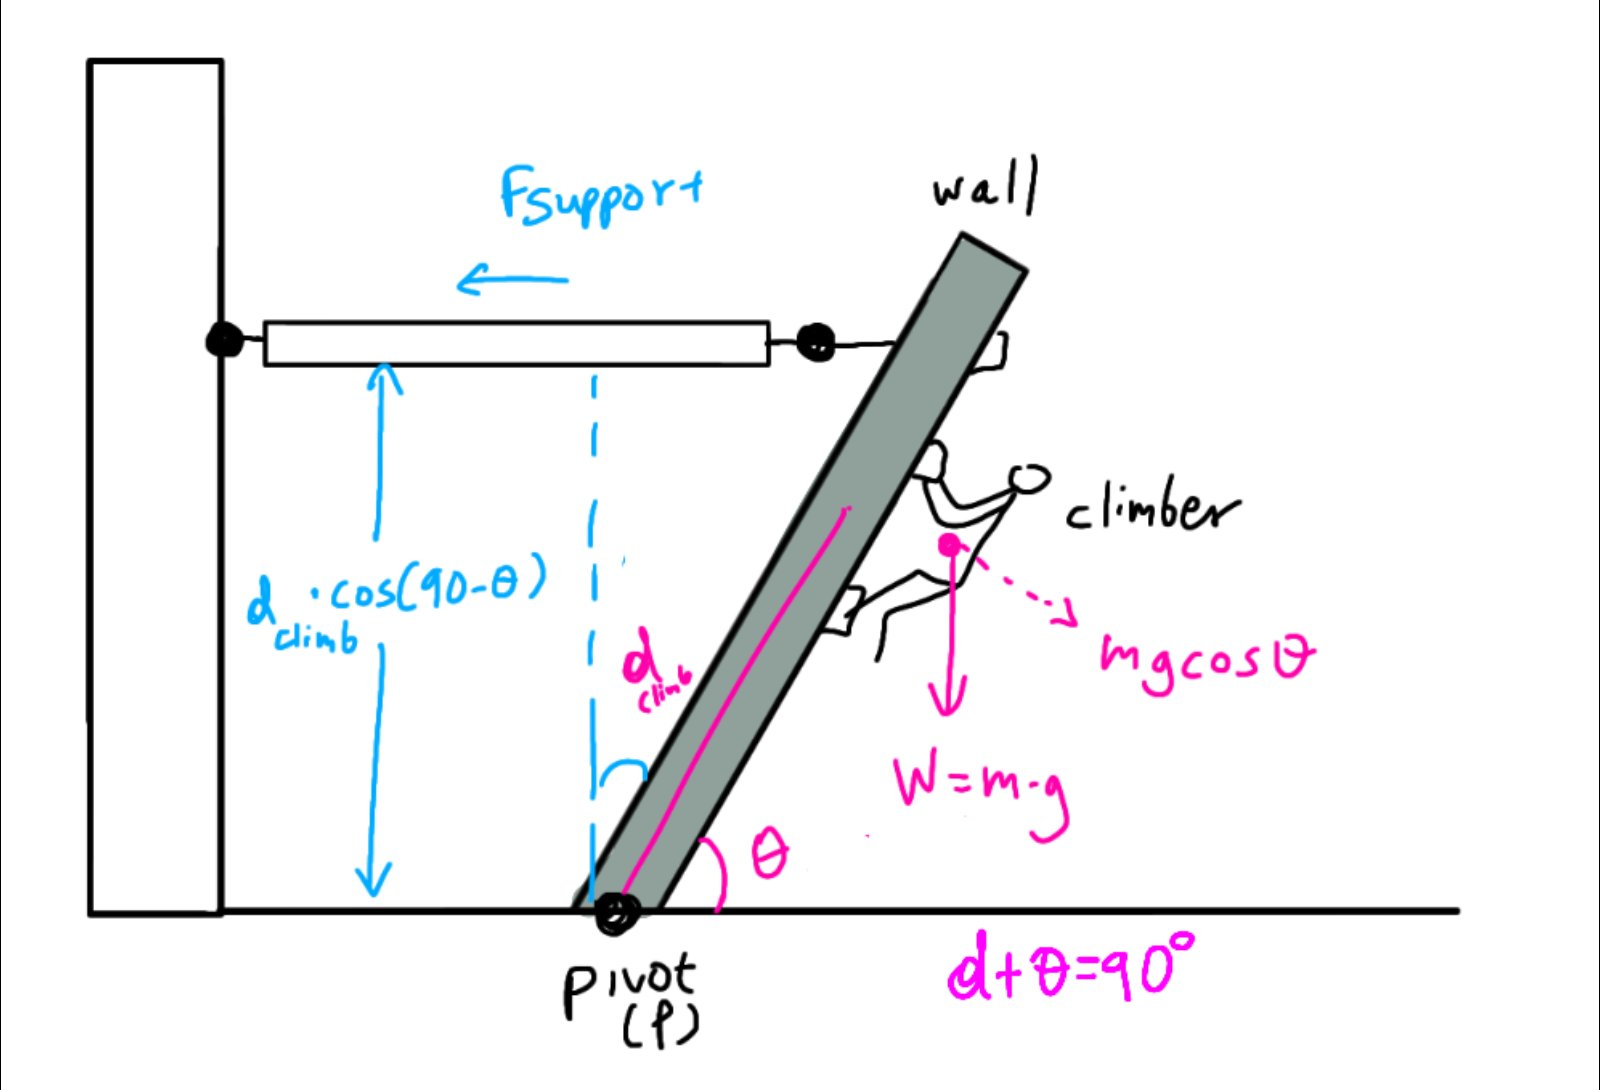
\includegraphics[width=0.75\linewidth]{752aa9dd-f1d8-445c-bf50-6b47ecbafaca.jpeg}
    \caption{Simplified Static Model}
    \label{fig:static}
\end{figure}

Worst case: climber at the top ($d = L$).

\[
\sum M_{\text{pivot}} = 0
\]
\[
\underbrace{F_{\text{support}} \cdot L \sin\theta}_{\substack{\text{restoring moment}\\\text{(straps pulling board back)}}}
=
\underbrace{m g \cdot L \cos\theta}_{\substack{\text{overturning moment}\\\text{(climber weight)}}}
+
\underbrace{M g \cdot \frac{L}{2} \cos\theta}_{\substack{\text{overturning moment}\\\text{(board weight at midpoint)}}}
\]

$L$ cancels:

\[
\boxed{F_{\text{support}} =
\underbrace{\left(m + \frac{M}{2}\right)}_{\substack{\text{climber mass +}\\\text{half board mass}}}
\times\;
\underbrace{g\vphantom{\frac{M}{2}}}_{\text{gravity}}
\times\;
\underbrace{\cot\theta\vphantom{\frac{M}{2}}}_{\substack{\text{geometry factor:}\\\text{flatter board}\\\text{= more force}}}
}
\]

\vspace{0.5em}
\textbf{Example:} $m = 100$ kg (climber), $M = 500$ kg (board), $\theta = 50^\circ$

\[
\cot(50^\circ) = 0.839
\]
\[
F_{\text{support}} = \left(100 + 250\right) \times 9.81 \times 0.839 \approx 2881\,\text{N}
\]

Split across three anchors:

\[
F_{\text{per anchor}} \approx 960\,\text{N}
\]

With a $3\times$ safety factor:

\[
F_{\text{per anchor, 3$\times$ SF}} \approx 2.9\,\text{kN}
\]

\textbf{This is a first approximation only.} It assumes the straps pull perfectly horizontally ($\phi = 0$) and attach at the very top of the board ($p = 1$). In reality, the straps angle downward about 10\textdegree{} and attach at 75\% of the board's length, both of which increase the forces. The generalised model in Section~\ref{sec:generalised} accounts for this.

% =====================================================

\section{Dynamic Forces During Climbing}
\label{sec:fall_impact}
During climbing, the forces on the board exceed the climber's static body weight. Push-offs during falls, dynamic moves (dynos), and cutting feet all produce force spikes.

\vspace{0.5em}
\begin{center}
\begin{tabular}{@{}lll@{}}
\toprule
\textbf{Scenario} & \textbf{Multiplier ($k$)} & \textbf{Force (100\,kg)} \\
\midrule
Static hanging & $1.0\times$ & 0.98\,kN \\
Steady climbing (moving between holds) & $1.2\text{--}1.5\times$ & 1.2--1.5\,kN \\
Push-off during fall & $\sim 1.5\text{--}2\times$ & $\sim$1.5--2.0\,kN \\
Dynamic move (dyno) & $2\text{--}3\times$ & 2.0--3.0\,kN \\
\bottomrule
\end{tabular}
\end{center}
\vspace{0.5em}

The dyno range is conservative: measured peak forces at the fingers reach 1.1--1.6$\times$ body weight ( see Notes); we round up to 2--3$\times$. The push-off estimate comes from a simple impulse calculation (100\,kg climber, $\sim$1\,m/s push-off over $\sim$0.2\,s $= 500$\,N, roughly half body weight on top of static), rounded up to $2\times$. The steady climbing range is not from a specific study; it sits between static and push-off as an engineering estimate, since each upward move briefly exceeds body weight as the climber accelerates between holds.

% =====================================================
\section{Generalised Static Model}
\label{sec:generalised}

The simplified model assumed ideal conditions: straps pulling horizontally from the very top of the board. In reality the straps attach at $p = 0.75$ of the way up (274~cm) and angle downward at $\phi \approx 10^\circ$ below horizontal. Both effects increase the strap force.

\begin{figure}[H]
    \centering
    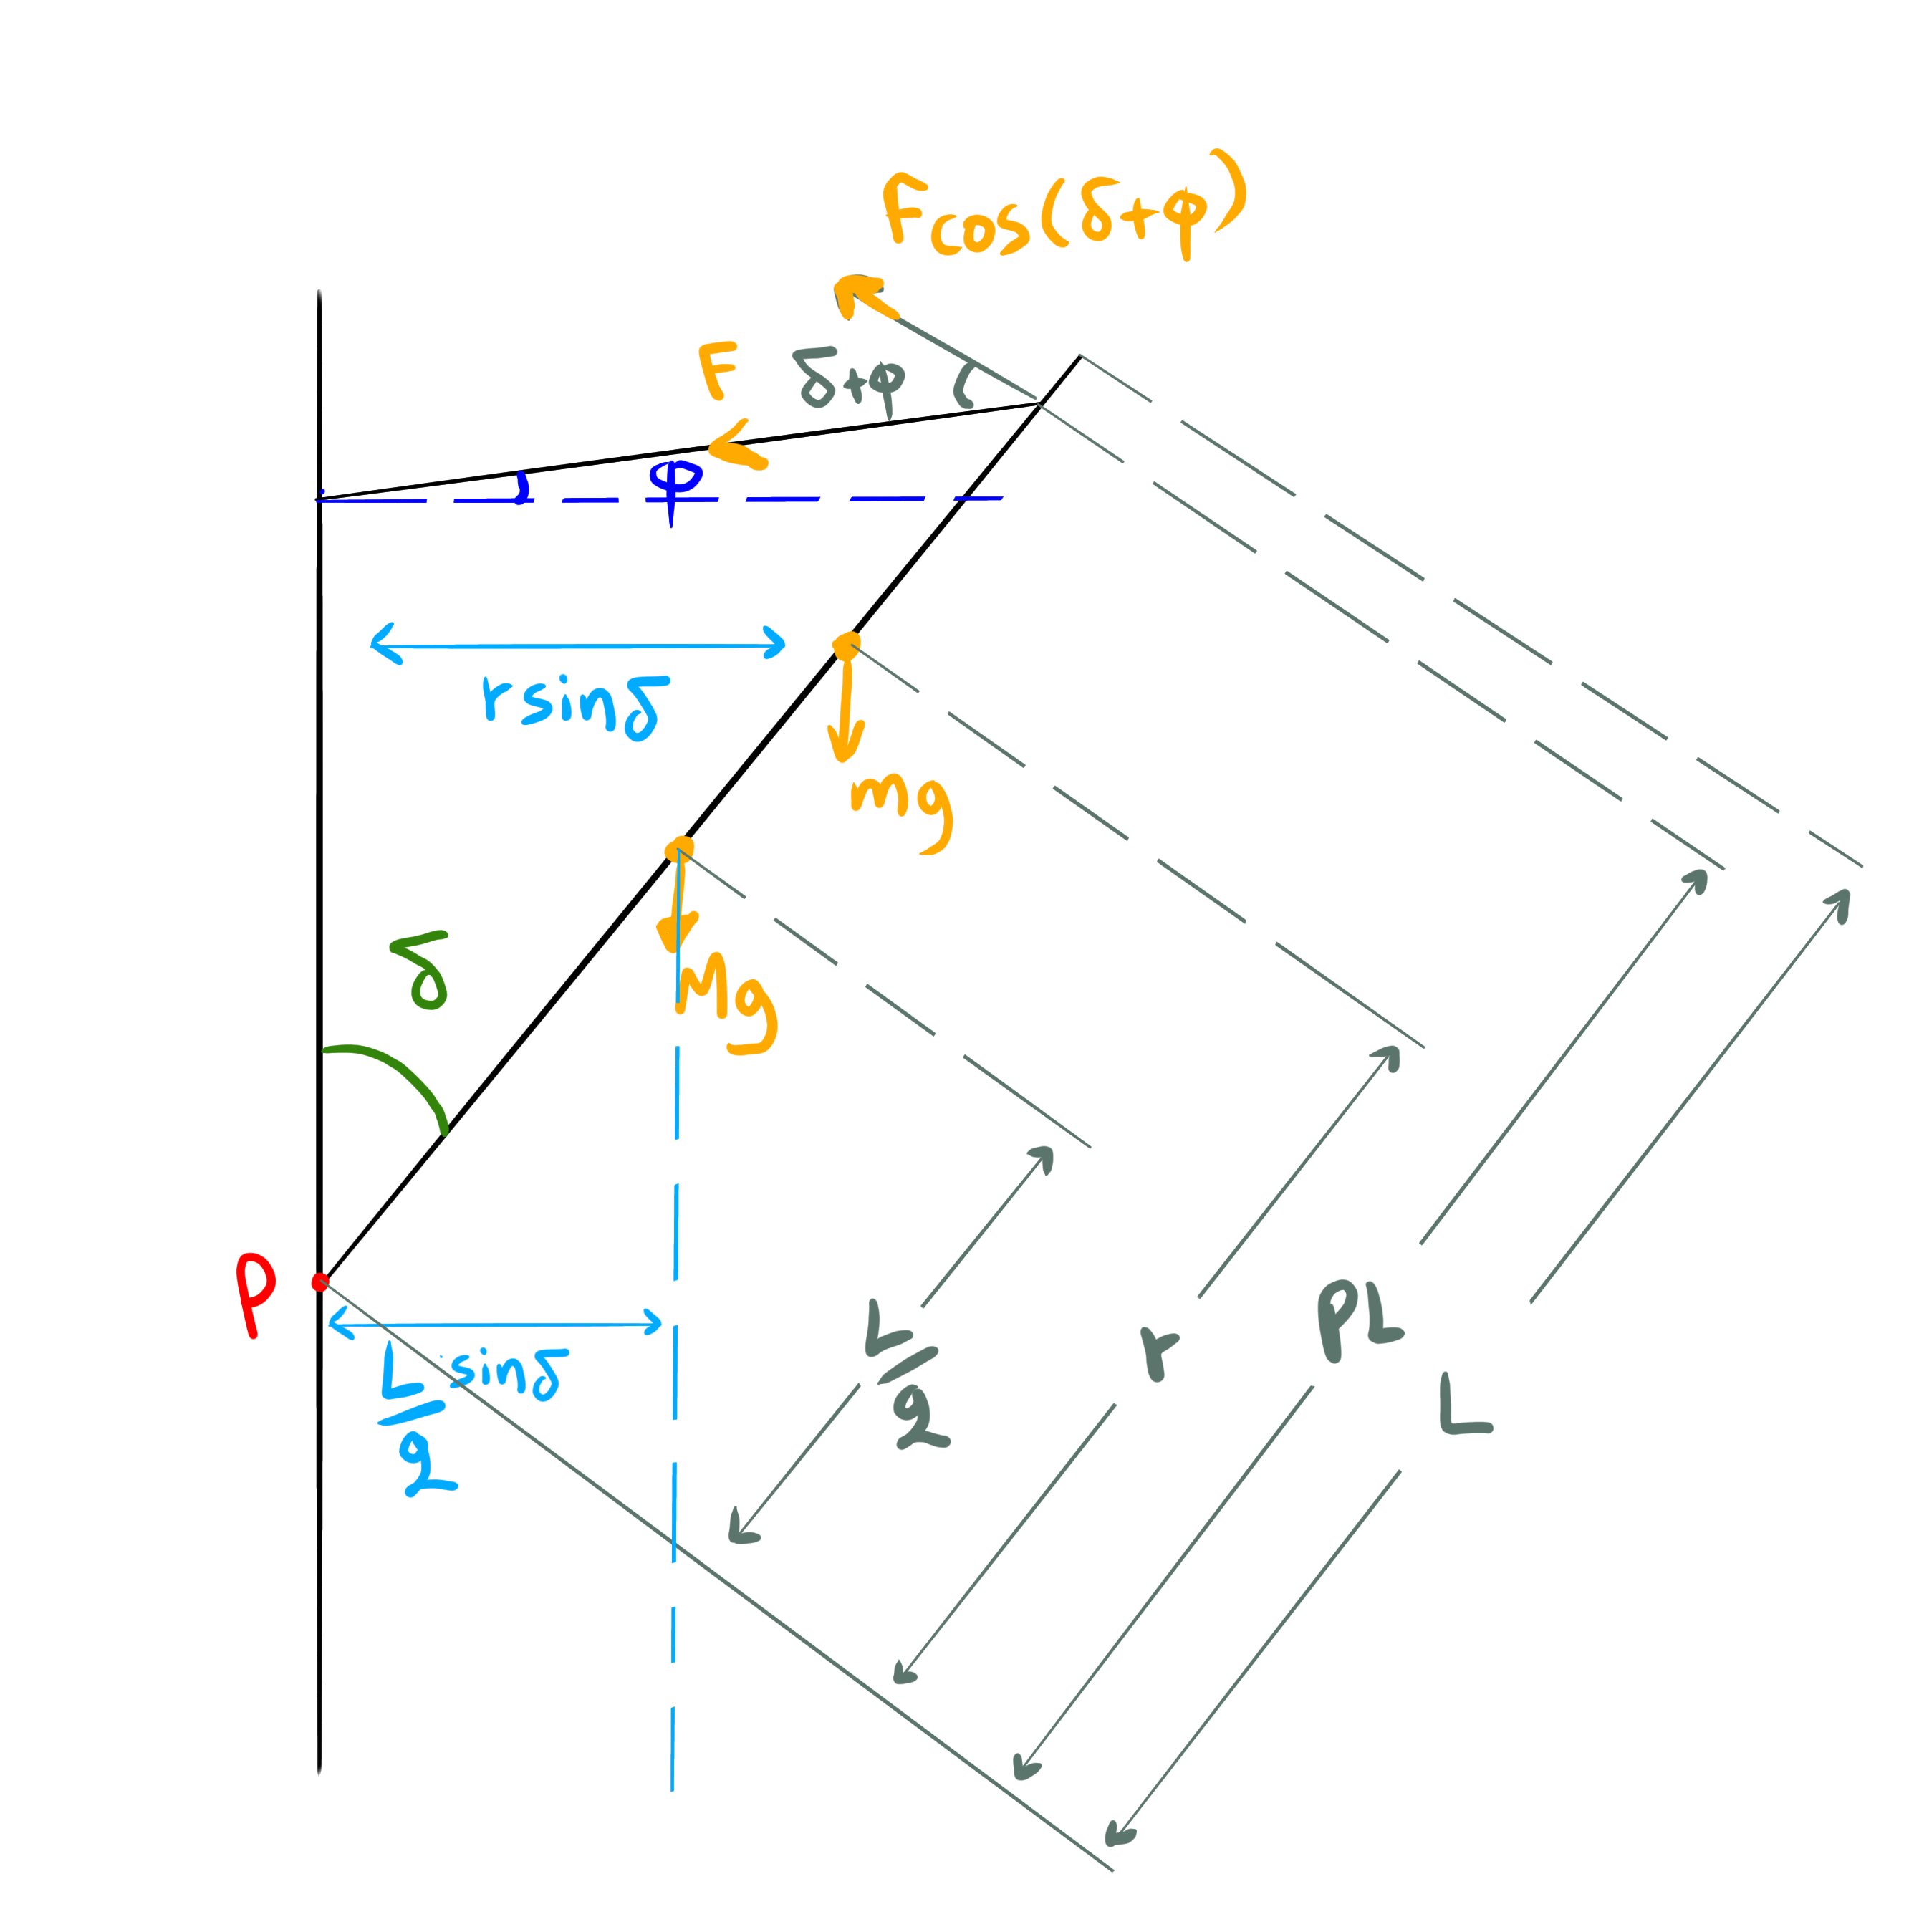
\includegraphics[width=0.75\linewidth]{graph_3.png}
    \caption{Generalised static model}
    \label{fig:generalised}
\end{figure}

\subsection{Defined Quantities}

\vspace{0.5em}
\begin{center}
\begin{tabular}{@{}ll@{}}
\toprule
\textbf{Symbol} & \textbf{Meaning} \\
\midrule
$M$ & Board mass (500 kg) \\
$m$ & Climber mass \\
$L$ & Board length (366 cm) \\
$r$ & Climber centre-of-mass distance from pivot \\
$\delta$ & Board inclination angle from vertical (40\textdegree) \\
$\phi$ & Strap angle below horizontal (10\textdegree) \\
$F$ & Total strap force \\
$p$ & Strap attachment fraction along board (0.75) \\
\bottomrule
\end{tabular}
\end{center}

\vspace{0.5em}
The value $p = 0.75$ follows from the measured strap length of 234~cm (centre), eye bolt height of 200~cm, and base offset of 54~cm. The strap angle $\phi \approx 10^\circ$ comes from the same geometry: the board attachment point sits about 42~cm above the eye bolt, over a horizontal run of 230~cm.

\subsection{Torques About the Pivot}

Moments about the base pivot:

\begin{itemize}
    \item Board weight (acting at $L/2$):
    \[
    \tau_{\text{board}} =
    \underbrace{Mg}_{\substack{\text{board}\\\text{weight}}}
    \cdot
    \underbrace{\frac{L}{2}}_{\substack{\text{acts at}\\\text{midpoint}}}
    \cdot
    \underbrace{\sin\delta}_{\substack{\text{perpendicular}\\\text{lever arm}}}
    \]

    \item Climber weight (acting at distance $r$ along the board):
    \[
    \tau_{\text{climber}} =
    \underbrace{mg}_{\substack{\text{climber}\\\text{weight}}}
    \cdot
    \underbrace{r\vphantom{\frac{L}{2}}}_{\substack{\text{distance}\\\text{from pivot}}}
    \cdot
    \underbrace{\sin\delta\vphantom{\frac{L}{2}}}_{\substack{\text{perpendicular}\\\text{lever arm}}}
    \]

    \item Strap force $F$ acts at distance $pL$ along the board. The angle between the strap force and the board is $(\delta + \phi)$, so the perpendicular moment arm is $pL \cos(\delta + \phi)$:
    \[
    \tau_{\text{strap}} =
    \underbrace{F\vphantom{pL}}_{\substack{\text{strap}\\\text{force}}}
    \cdot
    \underbrace{pL}_{\substack{\text{attachment}\\\text{distance}}}
    \cdot
    \underbrace{\cos(\delta + \phi)}_{\substack{\text{perpendicular}\\\text{component}}}
    \]
\end{itemize}

\subsection{Equilibrium}

Setting the restoring strap torque equal to the overturning torques:

\[
\underbrace{F \cdot pL \cos(\delta+\phi)}_{\text{restoring (straps)}}
=
\underbrace{mg \, r \sin\delta}_{\text{overturning (climber)}}
+
\underbrace{Mg \frac{L}{2} \sin\delta}_{\text{overturning (board)}}
\]

Solving for $F$, worst case with climber at the top ($r = L$, so $L$ cancels):

\[
\boxed{
F = \frac{
\overbrace{\left(m + \dfrac{M}{2}\right)}^{\substack{\text{effective}\\\text{mass}}}
\cdot\;
\overbrace{g \sin\delta}^{\substack{\text{gravity} \times \text{geometry}}}
}{
\underbrace{p}_{\substack{\text{attachment}\\\text{fraction}\\\text{(0.75)}}}
\;\cdot\;
\underbrace{\cos(\delta+\phi)}_{\substack{\text{strap angle}\\\text{penalty}\\\text{(reduces effectiveness)}}}
}
}
\]

\subsection{Dynamic Loading}
\label{sec:dynamic_loading}

To account for dynamic climbing forces, we replace the climber's static weight $mg$ with $k \cdot mg$, where $k$ is the amplification factor from Section~\ref{sec:fall_impact}:

\[
\boxed{
F = \frac{
\left(
\underbrace{k \, m \, r}_{\substack{\text{amplified}\\\text{climber load}}}
+\;
\underbrace{\dfrac{ML}{2}}_{\substack{\text{board load}\\\text{(unchanged)}}}
\right)
g \sin\delta
}{pL \cos(\delta+\phi)}
}
\]

% =====================================================
\newpage
\section{Board Bending \& Internal Forces}
\label{sec:bending}

\textit{Well...what if the board itself.. breaks?}

The board is held up at two points: the pivot at the bottom and the strap attachment at 75\% of the way up. Between and beyond those supports, the board carries load like a beam, but beams can bend, crack, or snap if the forces are too high.

Only the component of force \textit{perpendicular to the board} causes bending. For a board tilted 40\textdegree{} from vertical, that's $\sin(40^\circ) \approx 64\%$ of the total weight. The perpendicular self-weight is $w_\perp = 861$~N/m and the climber's perpendicular load is $F_{c,\perp} = k \times 631$~N.

\subsection{Where the Board Is Most Stressed}

Sweeping the climber across every position gives a bending moment \textit{envelope} the worst thing that can happen at every point along the board:

\begin{figure}[H]
    \centering
    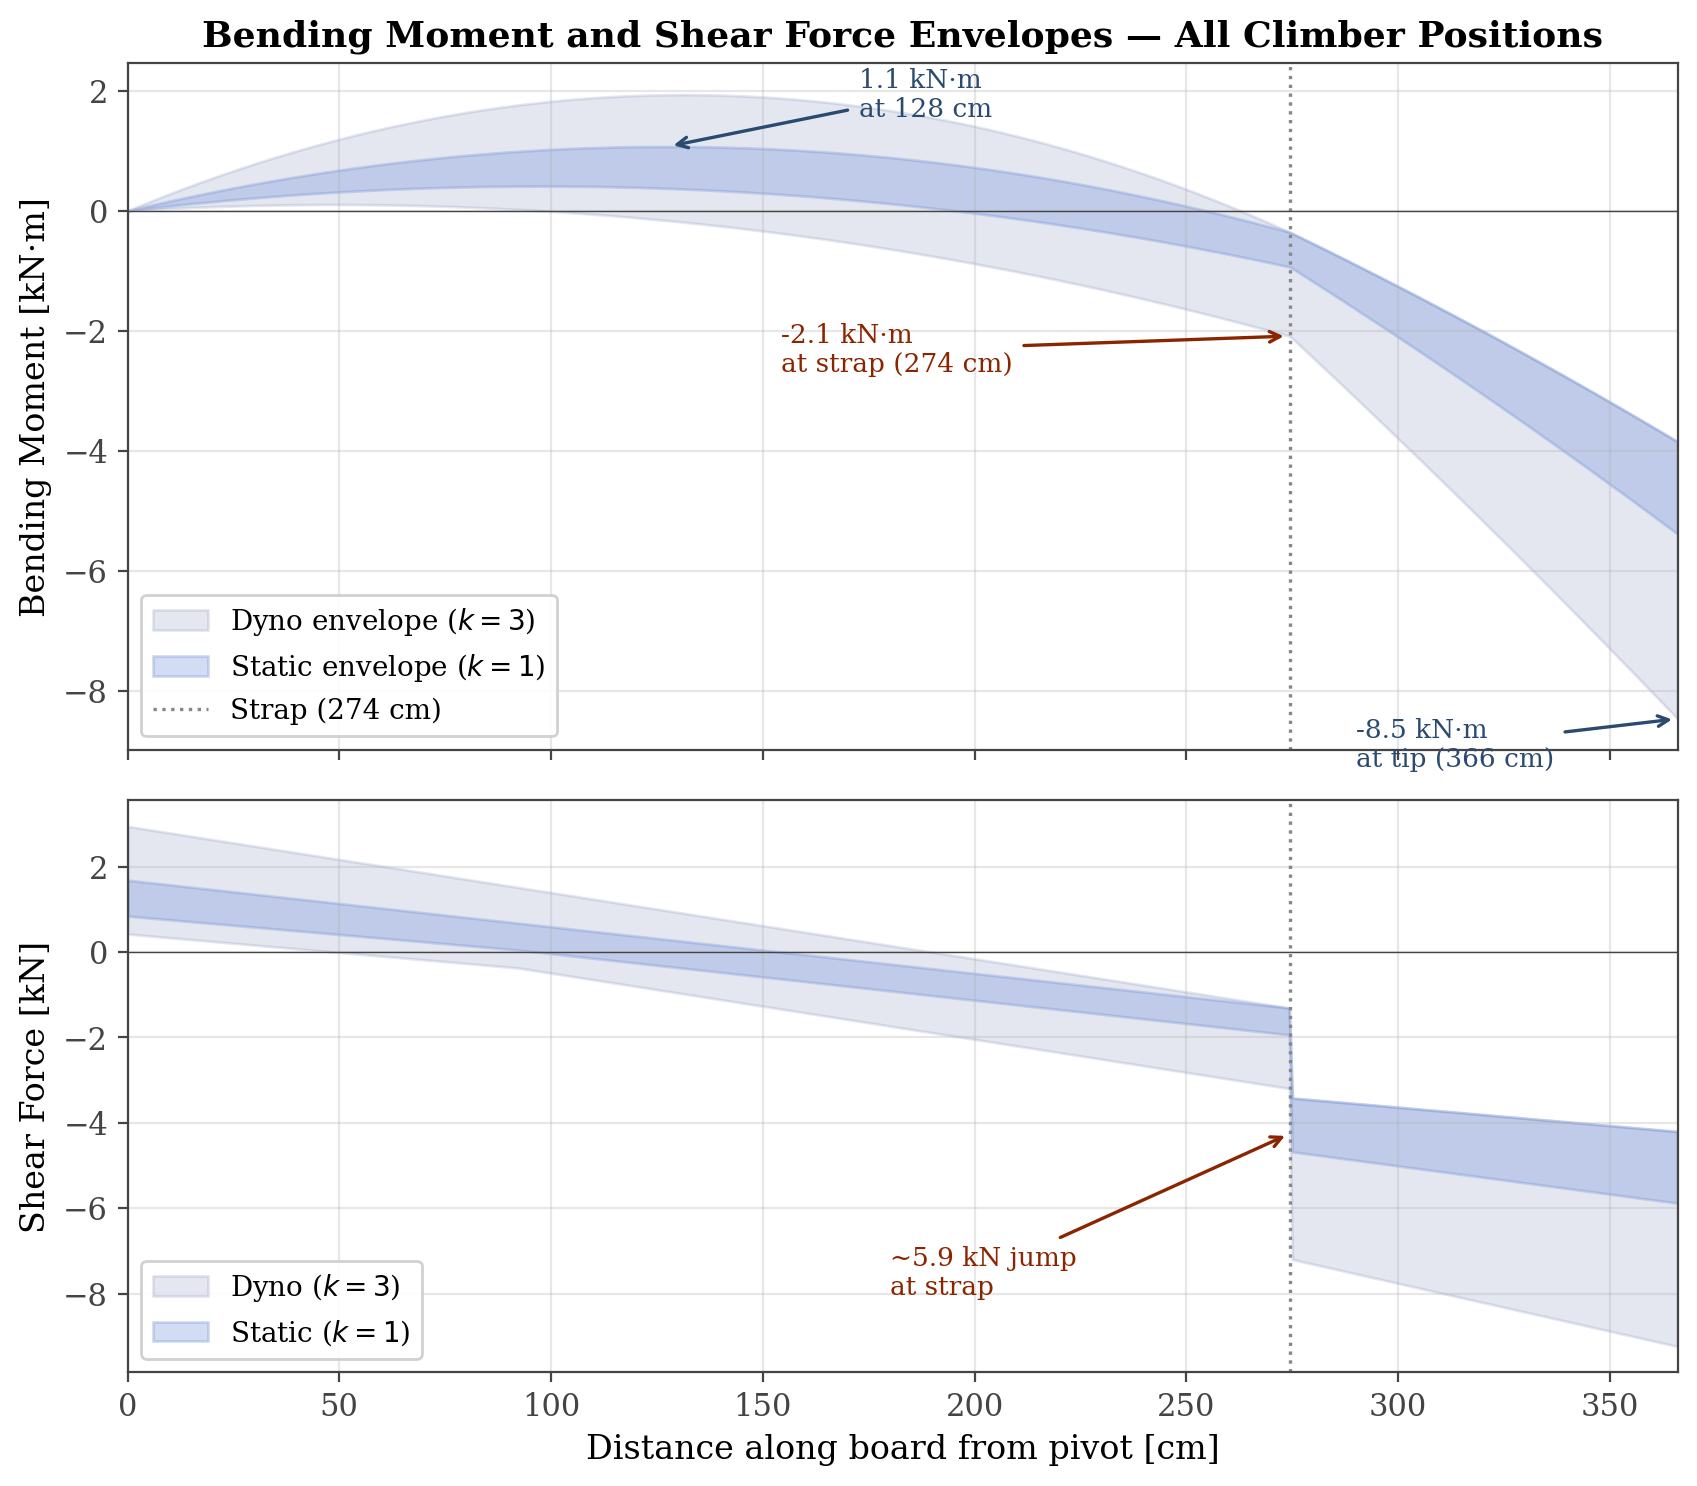
\includegraphics[width=0.92\linewidth]{bending_shear_envelope.png}
    \caption{Bending moment (top) and shear force (bottom) envelopes. The strap attachment at 274~cm is marked. The red annotation shows the worst \textit{hogging} (bending that tries to snap the board over the strap).}
    \label{fig:bending_shear}
\end{figure}

Two types of bending show up:

\begin{itemize}
    \item \textbf{Sagging} (positive moment): The board bows outward between the two supports. Worst case: $\approx$1{,}070~N$\cdot$m (static) at about 128~cm from the pivot.

    \item \textbf{Hogging} (negative moment): The board bends the \textit{other} way over the strap attachment. Worst case: $-$935~N$\cdot$m (static) right at the strap, rising to $-$2{,}089~N$\cdot$m under dyno loading ($k=3$).
\end{itemize}

\subsection{Peak Internal Forces}

\begin{table}[H]
\centering
\begin{tabular}{@{}lllll@{}}
\toprule
\textbf{Scenario} & \textbf{Max Bending} & \textbf{Where} & \textbf{Max Shear} & \textbf{Max Compression} \\
\midrule
Board only (no climber) & 641 N$\cdot$m  & 122 cm & 1.0 kN & 6.3 kN \\
Static ($k=1$)          & 935 N$\cdot$m  & at strap (274 cm) & 1.5 kN & 8.0 kN \\
Steady climbing ($k=1.5$) & 1{,}170 N$\cdot$m & at strap & 1.8 kN & 9.0 kN \\
Push-off ($k=2$)        & 1{,}400 N$\cdot$m & at strap & 2.1 kN & 10.0 kN \\
Dyno ($k=3$)            & 2{,}089 N$\cdot$m & at strap & 2.7 kN & 11.5 kN \\
\bottomrule
\end{tabular}
\caption{Peak internal forces. 100~kg climber at the top of the board ($r = L$).}
\label{tab:internal_forces}
\end{table}

\subsection{Critical Points on the Board}

\begin{enumerate}
    \item \textbf{Strap attachment (274~cm)}: \textit{the single most important location.} Highest bending moment, large shear jump, axial compression, and stress concentrations from bolt holes. Inspect this area first.

    \item \textbf{Mid-span ($\sim$128~cm)}: highest sagging moment. Any butt joints or plywood splices in the 80--180~cm zone are vulnerable.

    \item \textbf{Overhang (274--366~cm)}: the 91.5~cm cantilever above the straps. A climber here directly increases the hogging moment at the strap point below.

    \item \textbf{Pivot base (0~cm)}: zero bending, but the highest compression (8--11.5~kN). End-grain crushing is the risk.
\end{enumerate}

\subsection{Can the Board Handle It?}
\label{sec:section_check}

The board depth is 20~cm. The climbing surface width $b$ was not measured, but even a modest width produces very low stresses at this depth, because section modulus scales with $h^2$.

For a section $b \times 20$~cm under the worst dyno envelope ($M = 2{,}089$~N$\cdot$m, $N = 11{,}500$~N):

\[
\sigma = \frac{M}{Z} + \frac{N}{A}
= \frac{6 \times 2089}{b \times 0.20^2} + \frac{11500}{b \times 0.20}
= \frac{313\,350 + 57\,500}{b}
= \frac{370\,850}{b} \;\text{Pa}
\]

Even for a narrow board ($b = 0.5$~m), the combined stress is 0.74~MPa, compared to an allowable of $\sim$24~MPa for structural timber or $\sim$15~MPa for plywood. The board passes all loading scenarios by a very large margin, and bending is not a concern for this structure. The anchors and straps are the limiting components, not the board.

% =====================================================
\section{The Anchor Problem}
\label{sec:anchor_problem}

The wall is solid concrete block with rebar into a concrete base, extending 60~cm below grade.

Still, there are concerns. The render (plaster) is already cracking  around the anchors (Figure~\ref{fig:cracks}). The eye bolts are general-purpose hardware, not rated for life safety. UAE heat and UV degrade strap webbing over time, and thermal cycling can gradually loosen the anchors in the block. The centre strap is longer (234~cm vs 227~cm for the outer two) and the centre board anchor sits slightly higher, so load sharing between the three straps is unequal even before tensioning differences.

\begin{figure}[H]
    \centering
    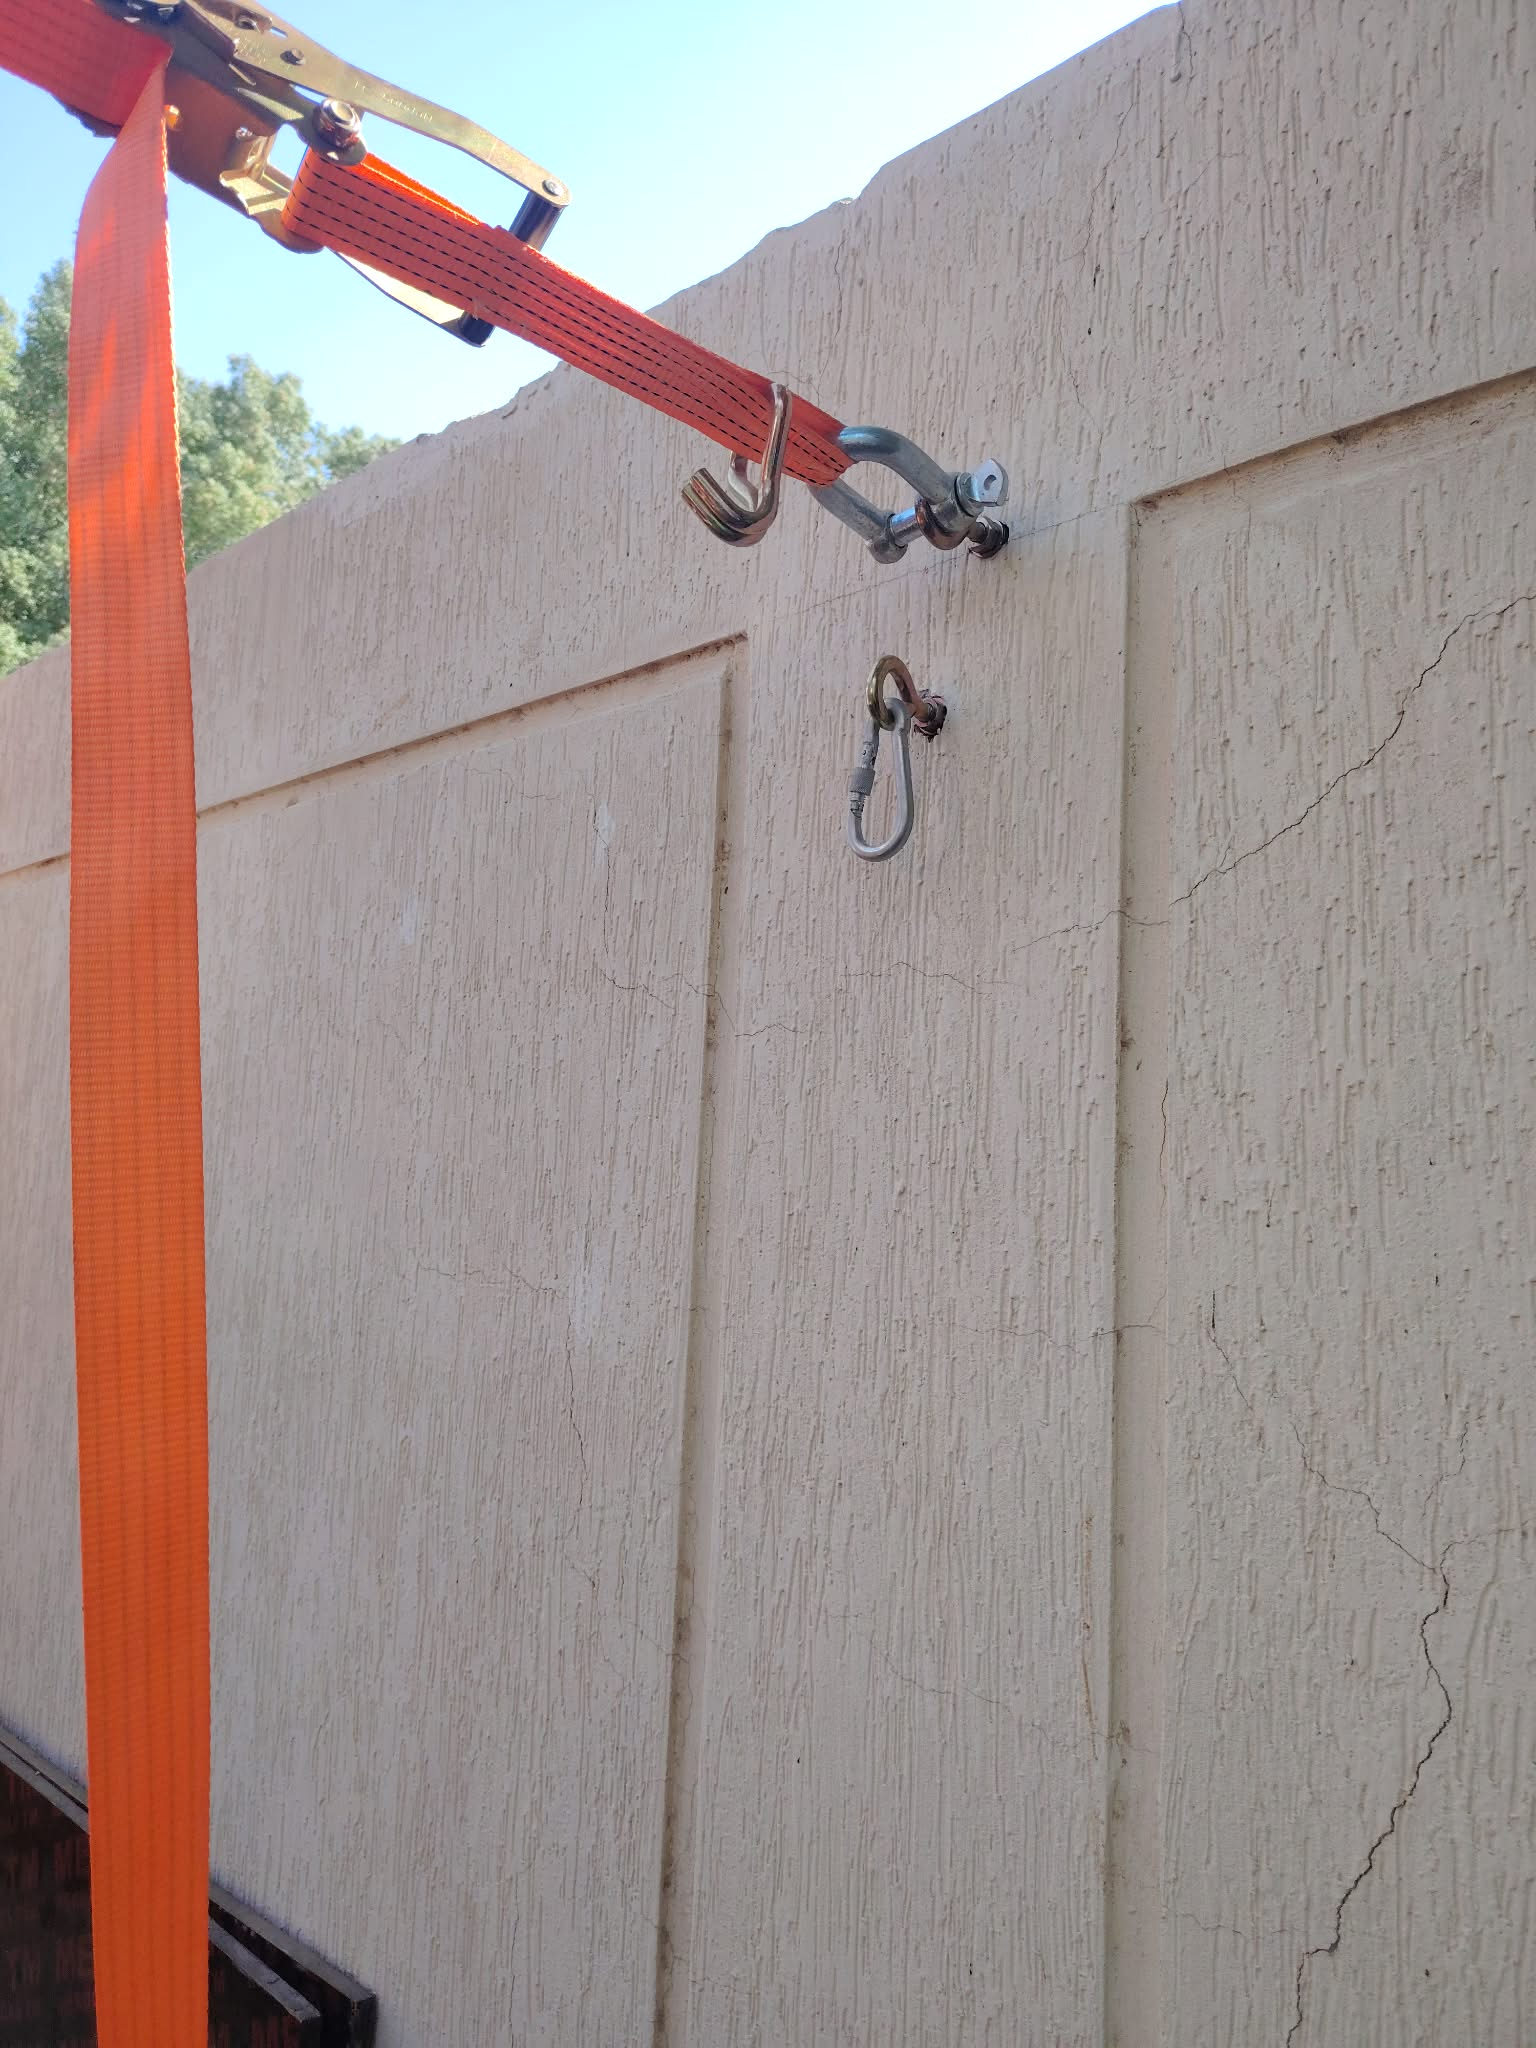
\includegraphics[width=0.5\linewidth]{wallcracks.jpeg}
    \caption{Wall has cracks visible already}
    \label{fig:cracks}
\end{figure}

Wall overturning was considered but requires the wall thickness to check properly. For a typical 200~mm reinforced block wall, self-weight and rebar should be sufficient at these loads.

\vspace{0.5em}
Recommended minimum anchor rating:

\[
\boxed{8\,\text{kN}}
\]

This gives margin above the $3\times$ static safety factor (4.58~kN per anchor) and covers all realistic dynamic climbing scenarios.
\newpage
% =====================================================
\section{Final Risk Estimation}
\label{sec:risk}

\begin{table}[h]
\centering
\begin{tabular}{l p{3.5cm} p{6.5cm}}
\hline
\textbf{Scenario} & \textbf{Per-anchor demand} & \textbf{Verdict} \\
\hline
Steady climbing, 500\,kg board & $\sim$1.7\,kN & Comfortable margin if anchors rated $\geq$ 8\,kN \\
Dynos ($k \approx 3$), 500\,kg board & $\sim$2.4\,kN & Still well within 8\,kN target \\
Steady climbing, 800\,kg board & $\sim$2.4\,kN (equal sharing); $\sim$3.6\,kN if one strap takes half & OK but less room for anchor degradation over time \\
Dynos ($k \approx 3$), 800\,kg board & $\sim$3.2\,kN (equal sharing); $\sim$4.8\,kN if one strap dominates & Tighter margin given existing wall cracks; hardware upgrades recommended \\
Long-term fatigue / unequal loading & Varies & The real concern; existing cracks may worsen with cycling, and one strap could briefly take most of the load \\
\hline
\end{tabular}
\caption{Final risk summary. 100\,kg climber at the top of the board.}
\label{tab:risk}
\end{table}

At 500~kg with equal load sharing, the system handles routine bouldering and dynos with comfortable margin, provided the anchors are rated $\geq 8\,\text{kN}$ and inspected regularly. At 800~kg the static numbers still look fine, but the margins depend heavily on how evenly the straps share load. With unequal sharing (likely, given different strap lengths and hand tensioning), a single anchor could see close to half the total force, and the existing wall cracks suggest anchor capacity may already be degrading.

\vspace{1em}
\textbf{The dominant practical risks are unequal strap loading and long-term fatigue, monitoring and hardware upgrades matter more than refining the static numbers.}

\vspace{0.5em}
\textbf{Real long-term and cumulative risks:}

\begin{itemize}
    \item \textbf{Anchor fatigue.} The wall already shows cracks around the anchors (Figure~\ref{fig:cracks}). Thousands of load cycles progressively loosen masonry anchors and propagate cracks, even at forces well below single-event capacity. Check regularly.

    \item \textbf{UV and thermal degradation.} Outdoor exposed polyester straps can lose $\sim$30\% of their strength in the first 12 months. UAE heat and thermal cycling also gradually loosen anchors. Replace straps at least annually.

    \item \textbf{Unequal strap loading.} The three straps are different lengths (234~cm vs 227~cm) and tensioned by hand. The tightest strap attracts the majority of the force. A single anchor could see well over a third of the total.

    \item \textbf{General-purpose hardware.} The eye bolts aren't rated for life safety. Upgrading to rated hardware with load distribution plates (Section~\ref{sec:load_plates}) would make a real difference.
\end{itemize}

Even unloaded, the board demands 3.27~kN from the straps, which leaves less reserve for dynamic events than a lighter board would. If anchor capacity degrades over time, the margin shrinks.

\newpage
% =====================================================
\section{Improvements}
\label{sec:improvements}

These are ideations I discussed with engineer friends that could potentially make the board more secure.

\subsection{A: Vertical Wire Rope with Diagonal Strut}
\label{sec:wire_rope}

\begin{figure}[H]
    \centering
    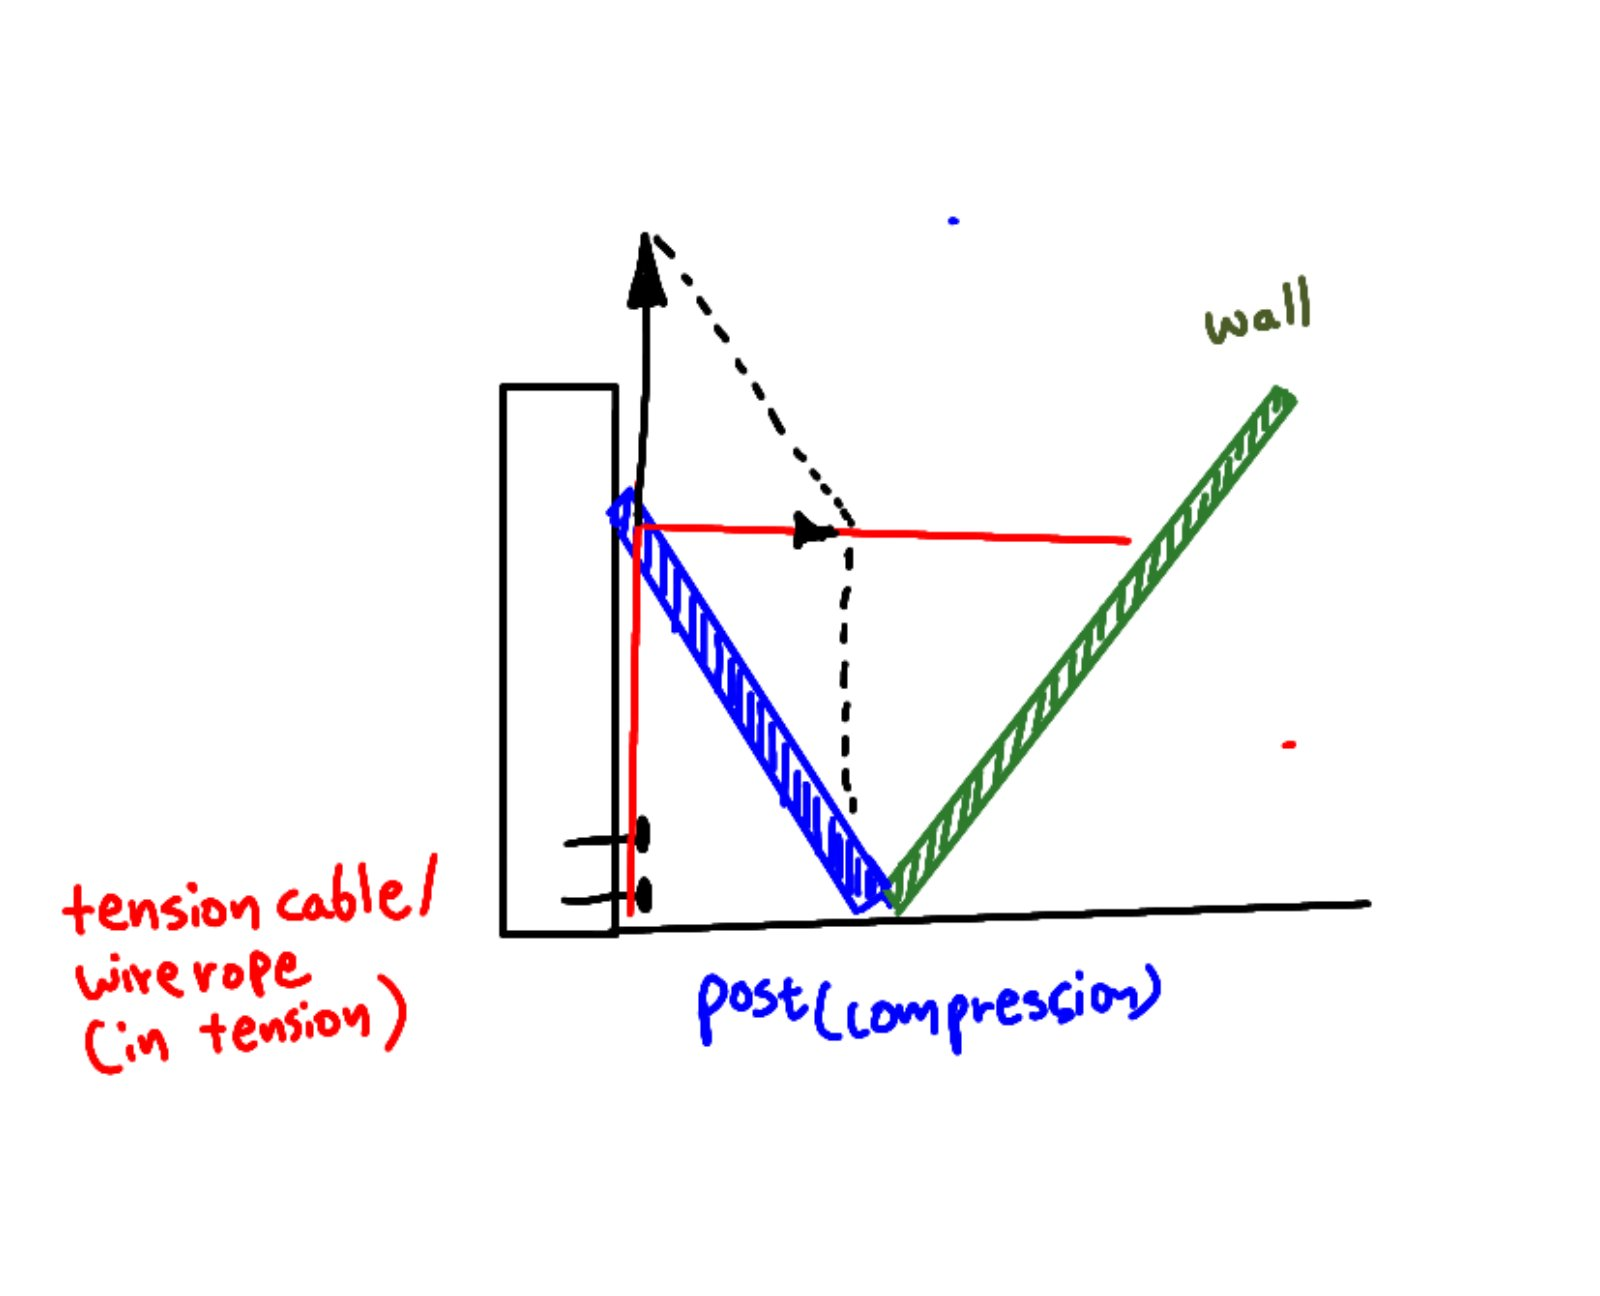
\includegraphics[width=0.75\linewidth]{fig5.jpeg}
    \caption{Post and tension cable}
    \label{fig:wire_rope}
\end{figure}

A heavy wire rope bolted vertically to the boundary wall at top and bottom, sitting flat against the wall surface. A diagonal steel or timber post connects from the wire rope to the base of the climbing board, working in compression.

The force from the climbing board splits vectorially: the vertical component goes into the wire rope (tension, transferred to the wall through top and bottom bolts), and the horizontal component goes into the diagonal post (compression, directed down to the base and into the ground).

It converts the loading on the wall from pure pull-out (the weakest mode) into a combination of shear and bearing, and uses the ground to carry the horizontal component through the compression strut.

\subsection{B: Fourth Strap Higher Up the Board}
\label{sec:fourth_strap}

All three straps attach at roughly the same height ($s \approx 274$~cm, or 75\% of the way up). Everything above that (91.5~cm) is an unsupported cantilever, and it's why Section~\ref{sec:bending} finds the worst bending moment right at $s = 274$~cm. A fourth strap higher up would split that cantilever into two shorter spans, cutting the peak bending moment. Same principle as a cable-stayed bridge (Figure~\ref{fig:cable_stayed}).

\begin{figure}[H]
    \centering
    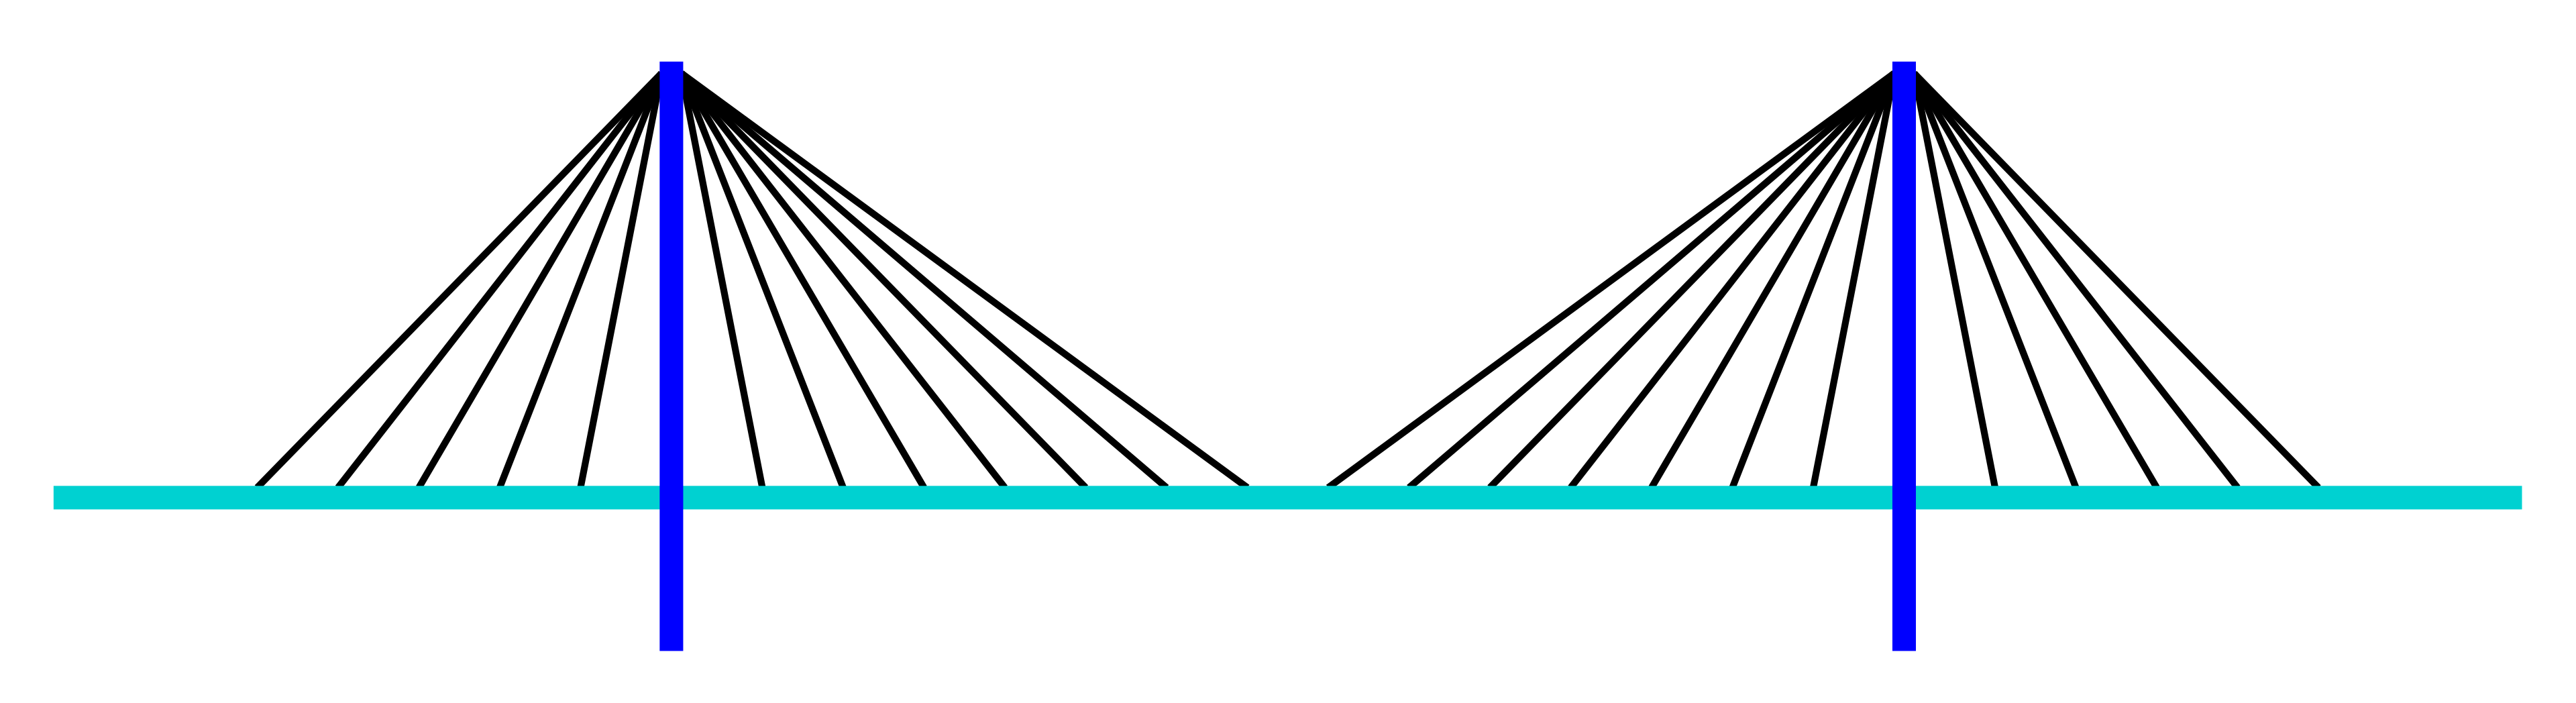
\includegraphics[width=0.65\linewidth]{cable_stayed_bridge.png}
    \caption{Cable-stayed bridge analogy. The wall is the tower, the board is the deck, and the straps are the stay cables. More attachment points means lower peak bending at any one section.}
    \label{fig:cable_stayed}
\end{figure}

Ideally as high as possible, but the board sits above the 226~cm wall top at $s \approx 330$~cm, so the practical limit is near the wall coping. Even cutting the cantilever from 91.5~cm to 60~cm helps proportionally. The trade-off is that higher attachment means a steeper strap angle, which reduces the strap's effectiveness, keep it below about 30\textdegree{} from horizontal.

\subsection{C: Load Distribution Plates}
\label{sec:load_plates}

Replace each single eye bolt with a steel plate secured by four anchors spaced approximately 20~cm apart. The pull-out force gets divided across four anchors instead of one, and spreading the anchors over a larger area reduces the chance of a single crack running through the wall. Chemical anchors are strongly recommended over mechanical expansion anchors for masonry.

\subsection{D: Pivot Base Plate}
\label{sec:base_plate}

Unsure if this was implemented already or not. The pivot base sees the highest axial compression on the board: 8.0~kN under static loading, rising to 11.5~kN during a dyno ($k=3$). All of this force funnels through the end grain of the wood onto the ground block, and end grain is the weakest orientation for crushing.

A steel bearing plate or hardwood block at the base would spread this load over a larger area. It also gives you an opportunity to bolt or pin the base to a ground plate, which would eliminate base sliding. The base currently rests on the ground with nothing fixing it in place, with the board weighing 500~kg the friction force is substantial ($\sim$2.5~kN at $\mu = 0.5$), but an aggressive lateral move could still overcome it.

\subsection{E: Equal-Length Straps}
\label{sec:equal_straps}

The centre strap is currently 234~cm while the outer two are 227~cm. That 7~cm difference means the shorter straps engage first and carry a disproportionate share. Making all three the same length removes this variable, though cranking three separate ratchets to exactly the same tightness is still practically impossible.

\vspace{0.5em}
\newpage
% =====================================================
\section{Limitations}
\label{sec:limitations}

This analysis is static-equivalent only; true transient response, vibration, and rate-dependent material behaviour are not modelled. No fatigue or cyclic assessment is included, though the existing crack pattern (Figure~\ref{fig:cracks}) may already evidence progressive damage. All forces assume equal load sharing across three straps. \textbf{In practice one anchor could briefly see close to the full load} and cascade failure if a strap or anchor lets go is not assessed. Lateral buckling of the board under compression, 3D strap geometry, and torsional effects are not analysed. All material properties are estimated from typical values, not tested. The climbing surface width was not measured; the section check in Section~\ref{sec:section_check} is parameterised in $b$ accordingly. Environmental degradation (UV, thermal cycling, creep) is noted but not projected over the service life.
% =====================================================
\section{Notes}
\label{sec:notes}

\noindent\textbf{1. Dyno forces (Section~\ref{sec:fall_impact})} \\[4pt]
\textit{Source: Fuss \& Niegl, ``Biomechanics of the two-handed dyno technique for sport climbing,'' Sports Engineering 13, 19--30 (2010).} \\[4pt]
Peak force at the fingers after touchdown ranged from 1.1 to 1.63 times body weight. I used 2--3$\times$ for overengineering.

\vspace{12pt}

\noindent\textbf{2. Strap degradation (Section~\ref{sec:anchor_problem})} \\[4pt]
Polyester webbing is rated for continuous use up to 100\textdegree C per BS EN 1492-1, so UAE ambient temperatures ($\sim$50--60\textdegree C surface) are within range. The greater concern is UV: outdoor-exposed polyester slings can lose $\sim$30\% strength in the first 12 months (Lift-It Manufacturing, \textit{Web Sling Product Information Bulletin}, \url{https://www.lift-it.com/pdf/Lift_It_Web_Sling_PIB.pdf}). Thermal cycling accelerates anchor loosening in masonry independently of strap strength.

\vspace{24pt}

\noindent\textbf{Thanks for reading :)}

\vspace{12pt}

\noindent By Stef.
\vspace{3pt}

\noindent Thank you Zac.

\noindent Also thanks for the help: Pi, Yiannis, Zulfy and Pepe (reviewing soon).
\end{document}
